\documentclass{beamer}
\usepackage{amsmath}
\usepackage{amsfonts}
\usepackage{amssymb}
\usepackage{polski}
\usepackage{pgfplots}
\pgfplotsset{compat=1.15}
\usepackage{mathrsfs}
\usetikzlibrary{arrows}
\usetheme{Warsaw}
\usefonttheme[onlymath]{serif}
\usepackage{animate}
\usepackage{caption}
\usepackage{graphicx}
\usepackage{booktabs}
\usepackage{tabularx}
\usepackage{overpic}
\renewcommand{\arraystretch}{1.5}
\beamertemplatenavigationsymbolsempty

\title{Być albo nie być czarną dziurą}
\author[F. Hansdorfer \and J. Winiarczyk \and Ł. Parda
\and T. Gruss]{Franciszek Hansdorfer \and Jacek Winiarczyk \and Łukasz Parda
\and Tomasz Gruss\\{\small Opiekun projektu: dr hab. Radosław Poleski}}
\date{\today}

\begin{document}

\begin{frame}
    \titlepage
\end{frame}

\section{Wprowadzenie do soczewkowania grawitacyjnego}
\subsection{Soczewkowanie grawitacyjne}

\begin{frame}
    \begin{columns}
        \begin{column}{0.5\linewidth}
            \begin{itemize}
                \item Ogólna teoria względności $\implies$
                \item Masa zakrzywia czasoprzestrzeń $\implies$
                \item Światło idące w pobliżu masy jest odchylane $\implies$
                \item Obserwator widzi obiekty za zakrzywiającą masą w inny sposób $\implies$
                \item Soczewkowanie grawitacyjne
            \end{itemize}
        \end{column}
        \begin{column}{0.5\linewidth}
            \begin{figure}
                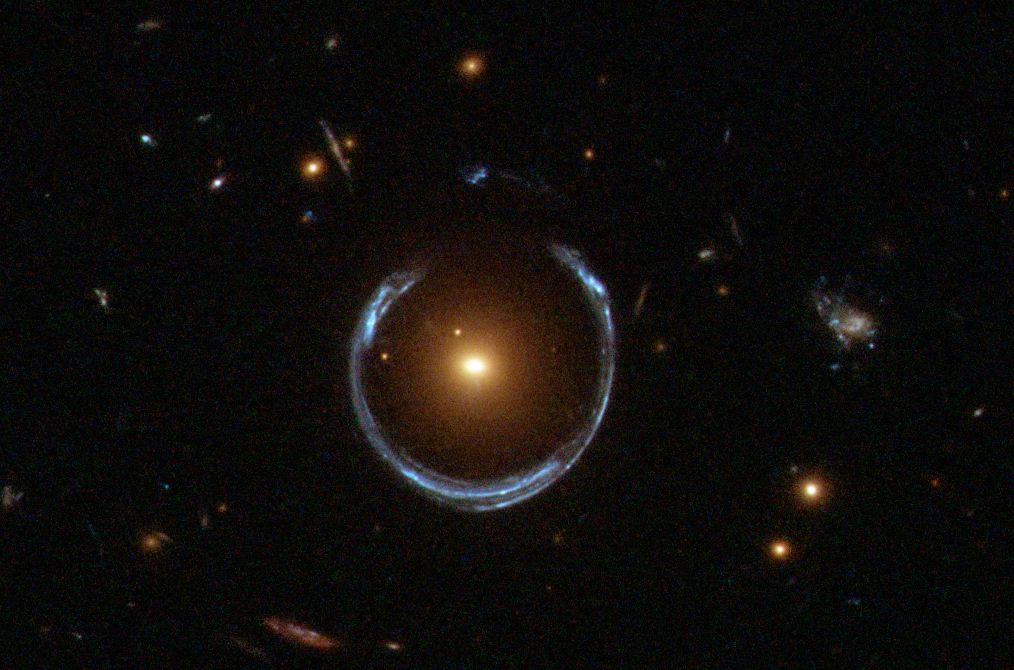
\includegraphics[width=\textwidth]{A_Horseshoe_Einstein_Ring_from_Hubble.jpeg}
                \caption*{\tiny{ESA/Hubble, NASA}}
            \end{figure}
        \end{column}
    \end{columns}
\end{frame}

\begin{frame}
    \begin{figure}
        \centering
        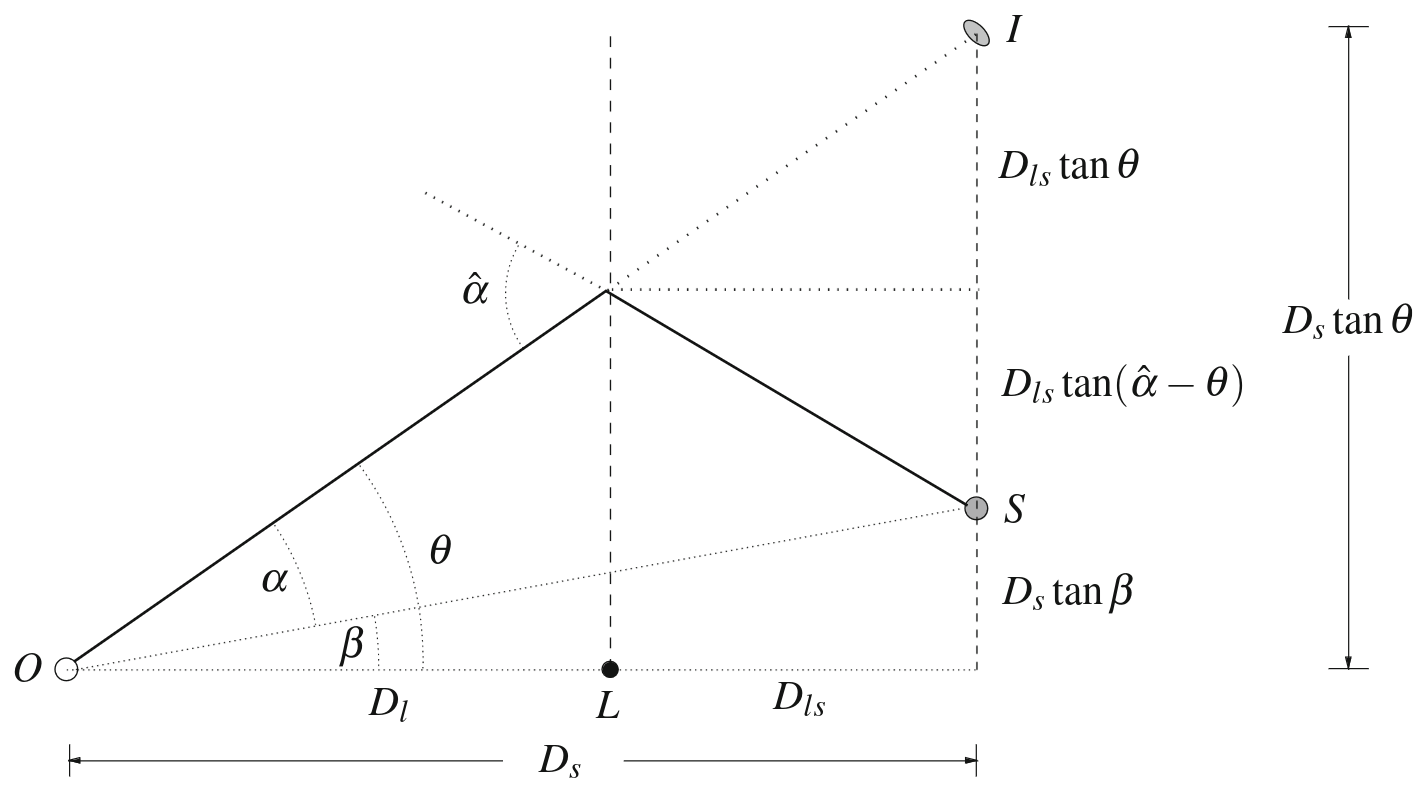
\includegraphics[width=0.6\textwidth]{Screenshot from 2024-06-10 13-41-41.png}
        \caption*{\tiny{Principles of Gravitational
                Lensing, Arthur B. Congdon, Charles R. Keeton}}
    \end{figure}
    \textbf{Równanie soczewki}:
    \[\beta = \theta - \alpha(\theta)\]
    Dla punktowej masy mamy:
    \[\theta_E = \sqrt{\frac{4GM}{c^2}\frac{D_s-D_l}{D_s D_l}}\]
\end{frame}

\subsection{Mikrosoczewkowanie}
\begin{frame}{Mikrosoczewkowanie}
    \begin{columns}
        \begin{column}{0.6\linewidth}
            \[M \sim M_{\odot}\]
            Na przykład dla $D_s = 8 \text{ kpc}$, $D_l = 4 \text{ kpc}$, $M = 1 M_{\odot}$:
            \[\theta_E = 0.32 \text{ mas}\]
            Dla $u = \frac{\beta}{\theta_E}$ wzmocnienie źródła określa wzór:
            \[A(u) = \frac{u^2 + 2}{u \sqrt{u^2 + 4}}\]
            $u$ możemy natomiast obliczyć znając $u_0, t_0, t_E$:
            \[u(t) = \sqrt{u_0^2 + \left(\frac{t-t_0}{t_E}\right)^2}\]
        \end{column}
        \begin{column}{0.4\linewidth}
            \begin{figure}
                \centering
                \animategraphics[width =\textwidth, loop, autoplay]{24}{animation1/Scott_Gaudi_anim-}{0}{65}
                \caption*{\tiny{Animation by B.S. Gaudi - microlensing-source.org}}
            \end{figure}
        \end{column}
    \end{columns}

\end{frame}

\subsection{Odchylenia od modelu punktowego źródła i soczewki}

\begin{frame}{Paralaksa}
    \begin{columns}
        \begin{column}{0.4\linewidth}
            Dla $t_{\text{E}}>30 \text{ d}$ ruchu Ziemi wokół Słońca przestaje być pomijalny. Wtedy:
            \begin{align*}
                 & u_{\oplus}(t) = u_{\odot}(t)+ \\&+\pi_{E}\beta\cos(\Omega(t-t_0)+\varphi)+\\&+\Lambda \omega(\sin(\Omega(t-t0)+\varphi))
            \end{align*}

        \end{column}

        \begin{column}{0.5\linewidth}
            \begin{figure}
                \centering
                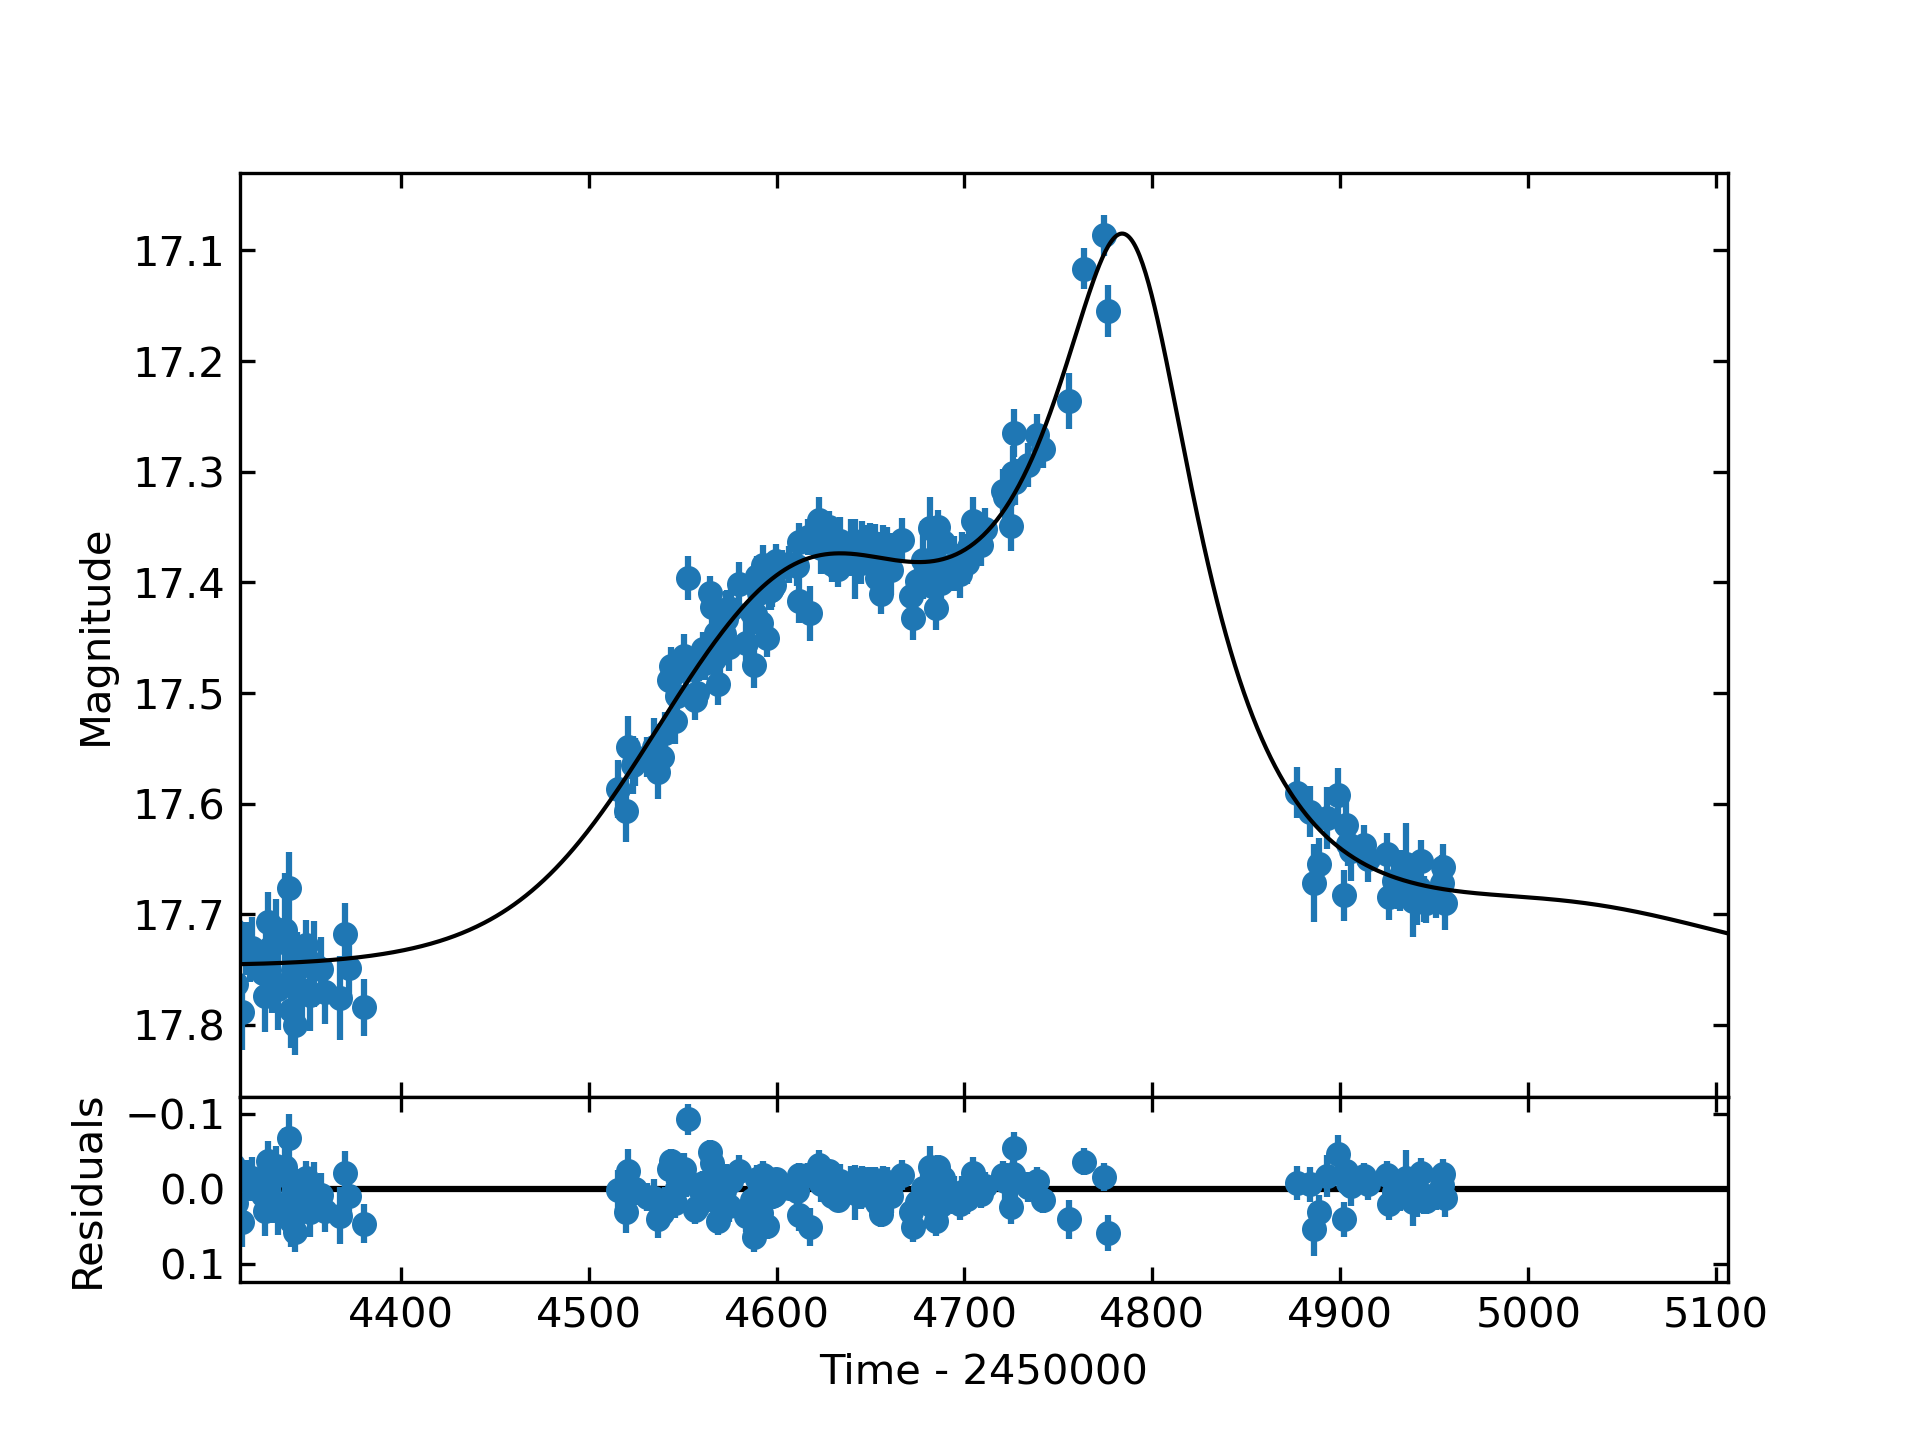
\includegraphics[width = \textwidth]{../sim30/parallax/png/PAR-20-noaver.dat-.png}
                \caption*{\tiny{PAR-20, $u_0<0$}}
            \end{figure}
        \end{column}
    \end{columns}

\end{frame}

\begin{frame}{Xallarap}
    \begin{columns}
        \begin{column}{0.5\linewidth}
            Jeżeli źródło jest częścią układu podwójnego, to jego ruch orbitalny może mieć znaczący wpływ na parametr $u(t)$.
            Ten feonomen nosi nazwę xallarap (Parallax od tyłu).
        \end{column}
        \begin{column}{0.5\linewidth}
            \begin{figure}
                \centering
                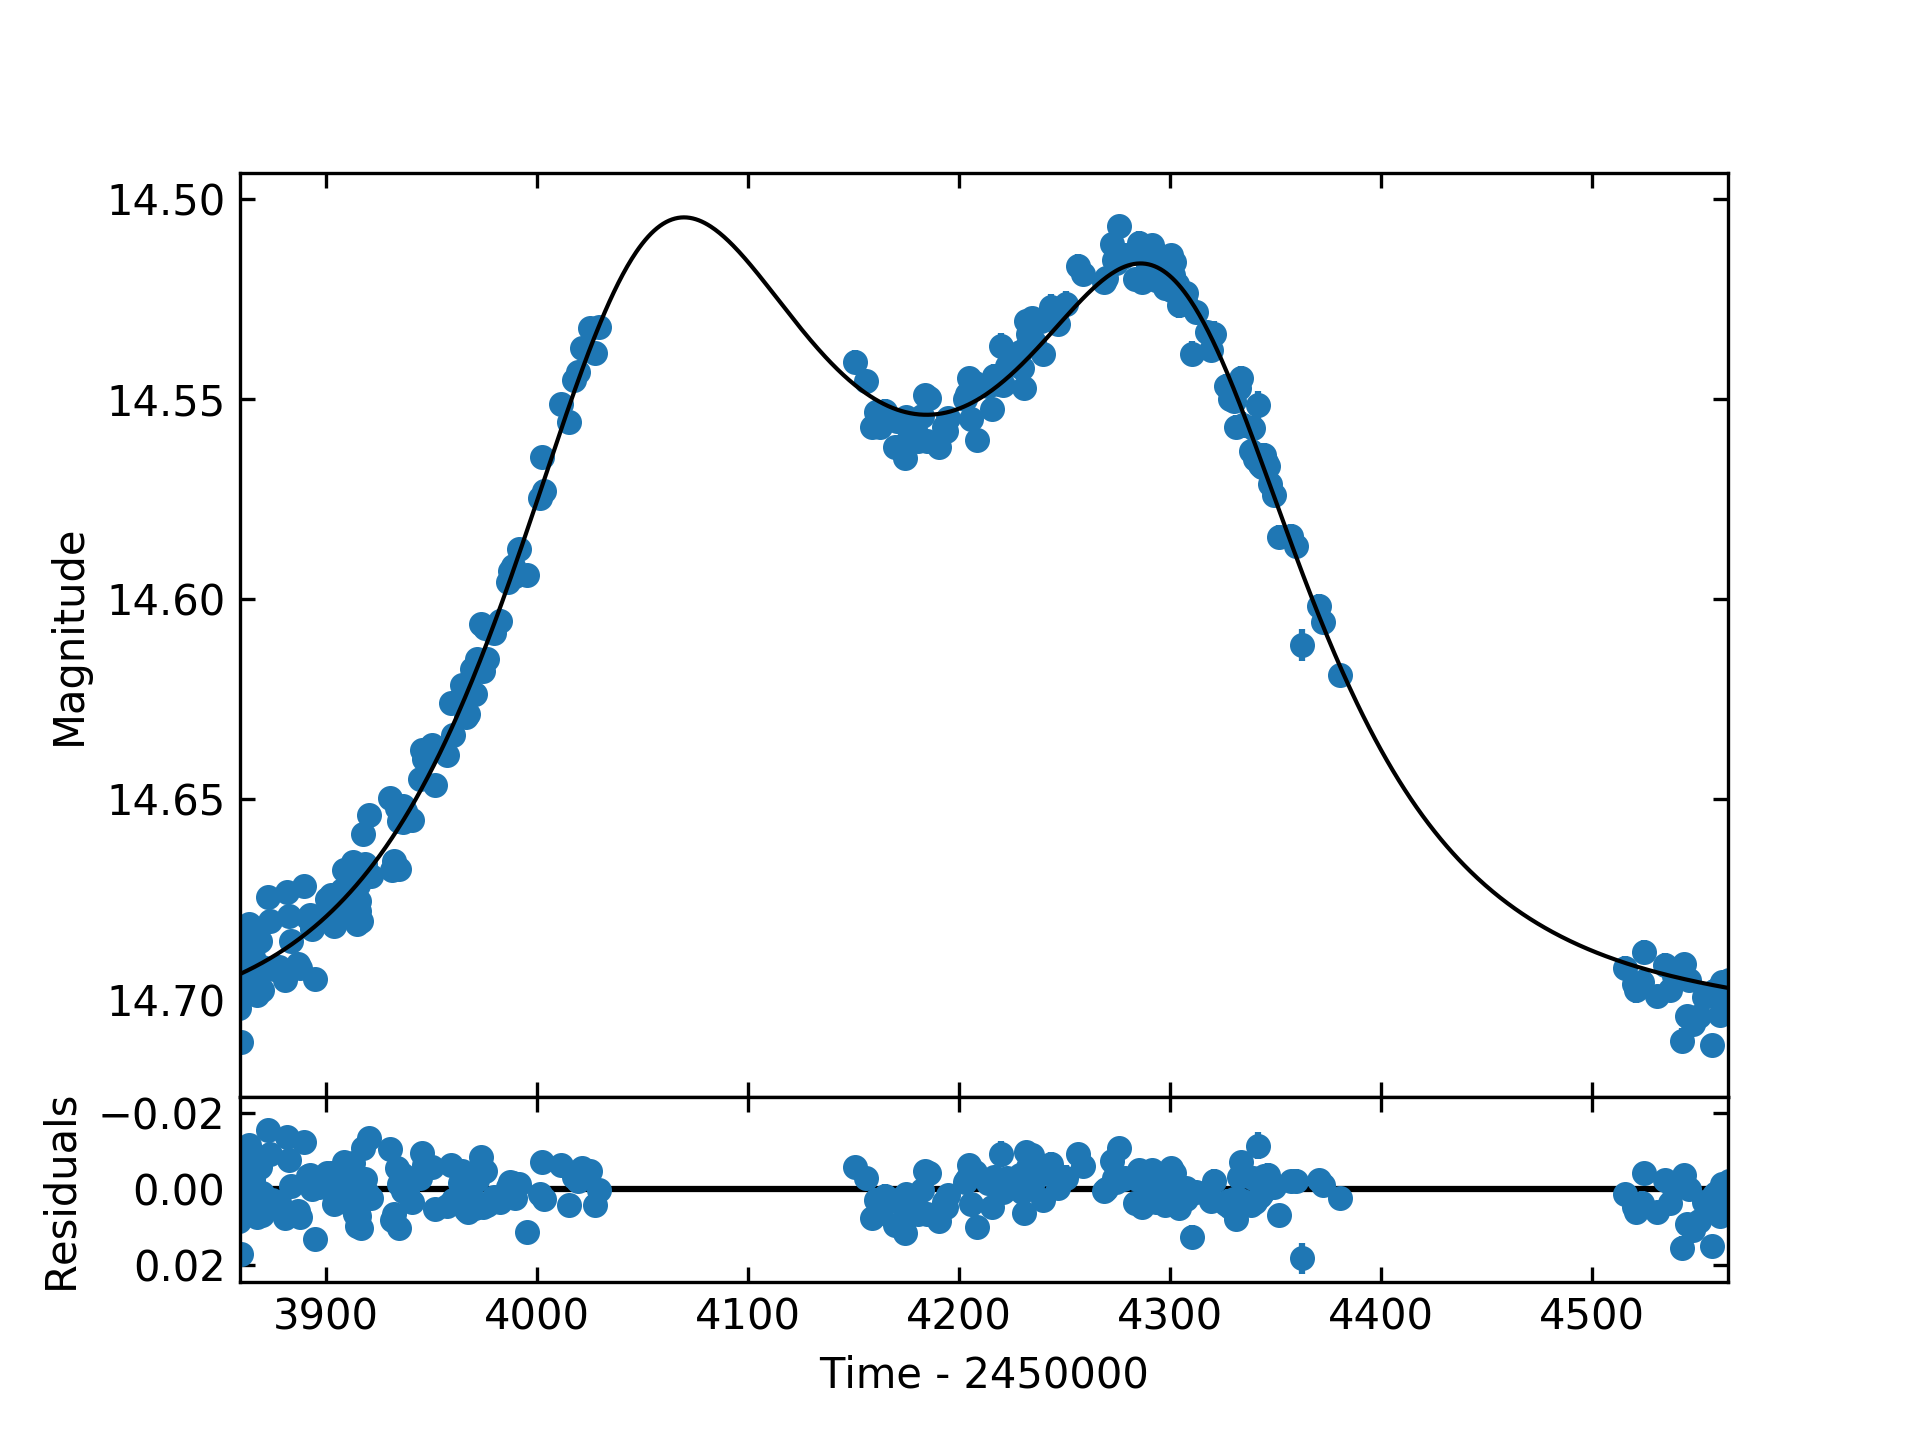
\includegraphics[width = \textwidth]{../sim30/xallarap/png/PAR-06-noaver.dat.10.png}
                \caption*{\tiny{PAR-06.10}}
            \end{figure}
        \end{column}
    \end{columns}
\end{frame}

\section{Modelowanie mikrosoczewkowania}
\subsection{MulensModel}
\begin{frame}
    \begin{columns}
        \begin{column}{0.5\linewidth}
            \emph{Mulens Model}, to paczka służąca do modelowania zjawisk mikrosoczewkowania.
            Do dopasowania krzywej, używany jest algorytm MCMC (Próbkowanie Monte Carlo łańcuchami Markowa).

        \end{column}

        \begin{column}{0.5\linewidth}
            \begin{figure}
                
\includegraphics[width = \textwidth]{logoMM_crop_4_372x260.png}
            \end{figure}
        \end{column}
    \end{columns}
\end{frame}

\section{Rezultaty}

\begin{frame}{Opis projektu}
    59 zjawisk wykazujących dominujący wpływ paralaksy(?), z przeglądu OGLE-III (Wyrzykowski et al. 2016).

    \bigskip
    \bigskip

    A co jeśli źródło jest w układzie podwójnym?
\end{frame}

\begin{frame}
    \centering
    \vspace{-0.25cm}
    \begin{columns}
        \begin{column}{0.5\linewidth}

            \begin{figure}
                \centering
                \begin{overpic}[width = \textwidth, keepaspectratio]{../sim30/parallax/png/PAR-06-noaver.dat+.png}
                    \put(40, 68){Parallax}
                \end{overpic}
            \end{figure}

        \end{column}
        \begin{column}{0.5\linewidth}

            \begin{figure}
                \centering
                \begin{overpic}[width = \textwidth, keepaspectratio]{../sim30/xallarap/png/PAR-06-noaver.dat.10.png}
                    \put(40, 68){Xallarap}
                \end{overpic}
            \end{figure}

        \end{column}
    \end{columns}

    \begin{figure}
        \centering
        \begin{overpic}[width = 0.5\textwidth, keepaspectratio]{../sim30/paraxall/png/PAR-06-noaver.dat+.png}
            \put(20, 68){ Parallax + Xallarap}
        \end{overpic}
    \end{figure}

\end{frame}

\begin{frame}{Porównanie modeli}
    \begin{table}[h]
        \centering
        \begin{tabularx}{\linewidth}{X r r}
            \toprule
            Nazwa  & $\Delta\chi^2$ & $\chi^2 _{Paraxall}$ \\
            \midrule
            PAR-05 & 52.7989        & 2360.0741            \\
            PAR-06 & 304.5130       & 4567.5600            \\
            PAR-14 & 37.3174        & 7164.3571            \\
            PAR-39 & 129.9147       & 13677.8037           \\
            PAR-57 & 59681.0222     & 4335.8364            \\
            PAR-58 & 34.7714        & 1087.9253            \\
            PAR-59 & 124.1144       & 2175.4949            \\
            \bottomrule
        \end{tabularx}
    \end{table}

\end{frame}

\begin{frame}{Wyniki}
    \begin{tabularx}{\linewidth}{X r r r}
        \toprule
        Nazwa       & $\xi_{period}$                & $\pi_{\text{EN}}$          & $\pi_{\text{EE}}$          \\
        OGLE-Ulens- & [days]                        &                            &                            \\
        \midrule
        PAR-05      & $600.151_{-80.54 } ^{+92.9}$  & $0.065_{-0.0 } ^{+0.02}$   & $0.065_{-0.0 } ^{+0.02}$   \\
        PAR-06      & $392.271_{-3.58 } ^{+3.46}$   & $-0.014_{-0.01 } ^{+0.02}$ & $-0.014_{-0.01 } ^{+0.02}$ \\
        PAR-14      & $314.276_{-11.7 } ^{+191.6}$  & $-0.553_{-0.04 } ^{+0.49}$ & $-0.553_{-0.04 } ^{+0.49}$ \\
        PAR-39      & $0.239_{-0.04 } ^{+0.87}$     & $0.032_{-0.0 } ^{+0.09}$   & $0.032_{-0.0 } ^{+0.09}$   \\
        PAR-57      & $0.692_{-0.11 } ^{+0.32}$     & $-0.012_{-0.03 } ^{+0.08}$ & $-0.012_{-0.03 } ^{+0.08}$ \\
        PAR-58      & $159.123_{-14.02 } ^{+10.96}$ & $-0.04_{-0.06 } ^{+0.08}$  & $-0.04_{-0.06 } ^{+0.08}$  \\
        PAR-59      & $16.886_{-0.95 } ^{+1.52}$    & $-0.566_{-0.22 } ^{+0.74}$ & $-0.566_{-0.22 } ^{+0.74}$ \\
        \bottomrule
    \end{tabularx}
\end{frame}

\begin{frame}{Dalsze kontynuacje badań}
    \begin{itemize}
        \item Wyznaczenie masy soczewek, dla których nasz model jest lepszy
        \item Ponowne wymodelowanie zjawisk, w celu zmniejszenia niepewności
        \item Zbadanie wpływu innych efektów na model (np. soczewka potrójna)
    \end{itemize}
\end{frame}

\end{document}